\begin{refsection}

\hypertarget{discussion-guxe9nuxe9rale-et-perspectives}{%
\chapter{Discussion Générale et
Perspectives}\label{discussion-guxe9nuxe9rale-et-perspectives}}

L'objectif général de ce travail de thèse est d'améliorer notre
compréhension des processus régissant la distribution des habitats
benthiques biogéniques et de leurs communautés associées. Pour ce faire,
dans le premier chapitre de ce manuscrit, j'ai étudié les règles
d'assemblage dans une communauté benthique structurée par deux habitats
distincts; dans le second chapitre, j'ai identifié et caractérisé des
états d'habitats biogéniques à l'échelle du globe et enfin, dans le
dernier chapitre j'ai identifié les facteurs qui contrôlent la
distribution spatiale de ces états d'habitats. Etant donné le rôle
important de ces habitats pour maintenir la biodiversité des écosystèmes
côtiers, ces travaux permettent de mieux envisager leur réponse face aux
changements environnementaux en cours et les effets cascades qui peuvent
en découler sur la biodiversité et le fonctionnement des écosystèmes
côtiers.

\hypertarget{amuxe9liorer-les-capacituxe9s-pruxe9dictives-des-moduxe8les-de-distribution-despuxe8ces}{%
\section{Améliorer les Capacités Prédictives des Modèles de \\Distribution
d'Espèces}\label{amuxe9liorer-les-capacituxe9s-pruxe9dictives-des-moduxe8les-de-distribution-despuxe8ces}}

L'un des principaux objectifs de cette thèse était de comprendre et de
prédire les réponses des communautés benthiques côtières. À cet effet,
j'ai employé deux méthodes distinctes de prédictions. Dans le premier
chapitre, j'ai adopté l'approche ``\emph{prédire et aggréger
simultanément}'' selon \textcite{Ferrier_2006} en utilisant un
\emph{jSDM} \autocite{Warton_2015}. Dans le deuxième et troisième
chapitre, j'ai employé une approche ``\emph{grouper, puis prédire}''.
Ces stratégies ont chacune montré leurs avantages et leurs limites. Les
résultats du premier chapitre ont indiqué que l'intégration
d'informations supplémentaires, comme la phylogénie ou d'autres espèces
associées, renforçait la performance prédictive. Cependant, l'ajout de
traits fonctionnels n'a pas consolidé les performances prédictives de
l'approche, allant au contraire de ce qui est attendu dans ce genre de
modèle \autocites[ ]{Ovaskainen_2017a}{Ovaskainen_2020}. Cela semble
suggérer que les traits sélectionnés pour la communauté de polychètes
n'étaient pas suffisamment en lien avec les conditions environnementales
du modèle et que par conséquent, les liens traits-environnement ne
permettaient pas d'informer suffisamment le modèle pour améliorer ses
prédictions. Ainsi, savoir si l'on a utilisé les ``bons'' traits
d'espèces reste encore une question cruciale pour obtenir le meilleur
pouvoir prédictif d'un \emph{SDM} ou \emph{jSDM} \autocite{Vesk_2021}.

Face à des résultats prédictifs qui ne répondaient pas à mes attentes et
à une interprétabilité limitée par le nombre d'espèces en jeu, j'ai
formulé une nouvelle méthode dans les chapitres 2 et 3. Au lieu de
chercher à prédire la totalité de la communauté, j'ai considéré
l'utilisation de proxys pour améliorer le pouvoir prédictif des modèles.
J'ai ainsi choisi l'approche ``\emph{grouper, puis prédire}'' de
\textcite{Ferrier_2006} en me servant des habitats biogéniques et de
leurs états possibles comme proxys des communautés benthiques et de la
biodiversité côtière \autocite{PelletierD_2020}. L'étendue des habitats
biogéniques est depuis longtemps utilisée comme proxy de l'état des
écosystèmes marins, à l'échelle globale \autocite{Stuart_2010}, mais
leur étendue seule n'est pas suffisante, car, selon leur état, ces
habitats n'abritent pas le même niveau de diversité
\autocite{Sunday_2017}. J'ai donc exploré la prédictibilité et la
réponse aux changements environnementaux de ces habitats biogéniques et
de leurs différents états possibles. Cependant, cette tentative n'a pas
non plus rencontré le succès escompté. Au-delà des questions soulevées
par le chapitre 2 quant aux méthodes pour définir et classifier les
habitats benthiques et leurs états, le chapitre 3 a montré que la
prédictibilité de ces états d'habitats reste faible. Le chapitre 3
discute des facteurs qui peuvent limiter la prédictibilité d'états
écologiques, mais il convient de revenir sur des points transverses avec
le chapitre 1, car il existe des facteurs qui limitent la prédictibilité
et transférabilité de tous modèles de distribution d'espèces
\autocite{Yates_2018}.

Prédire en écologie s'avère complexe, notamment lors de l'étude de
communautés entières ou à de vastes échelles spatio-temporelles.
Néanmoins, cette thèse a mis en lumière diverses pistes de réflexion
pour optimiser les prédictions. Une préoccupation majeure est la
résolution des données environnementales relativement à l'écologie des
espèces modélisées. En effet, les données environnementales utilisées
comme co-variables sont souvent disponibles à des échelles grossières et
trop larges relativement à la taille des organismes étudiés
\autocite{Potter_2013}. Par exemple, les données environnementales
terrestres bénéficient d'une résolution d'environ 1 km, à l'instar de la
base de données \emph{Chelsea} \autocite{Karger_2017}, cette résolution
n'est que d'environ 9 km pour Bio-Oracle en milieu marin
\autocite{Assis_2018}, alors que l'ordre de grandeur des espèces
associées aux écosystèmes étudiées dans cette thèse ont des ordres de
grandeur inférieurs au mètre. Cette discordance limite les capacités
prédictives des modèles en réduisant la variabilité spatiale des
conditions environnementales qu'expérimentent réellement ces espèces.
Ainsi, lors de l'entraînement des modèles de distribution d'espèces,
nous n'avons accès qu'à une partie tronquée de leurs niches réalisées.
Une piste prometteuse serait d'intégrer les conditions microclimatiques
qui expérimentent les communautés. Pour ce faire, il est possible
d'envisager des loggeurs \emph{in situ} \autocite{Lembrechts_2019}, mais
cette solution n'est pas réalisable pour les suivis à grande échelle
spatiale. Des approches numériques pourraient améliorer notre
appréhension des variations climatiques à une échelle spatiale bien plus
fine : à l'aide d'approches numériques, via des approches mécanistiques
telles que celles présentées par \textcite{Maclean_2019} ou des
approches par réseaux de neurones telles que celles présentées par
\textcite{Hu_2023}, il est possible de reconstruire les conditions
climatiques a fine échelle, de l'ordre de 100 m$^{2}$, voir jusqu'à 10
m$^{2}$ \autocite{Maclean_2020}. Ces approches ont déjà été testées sur
certains écosystèmes terrestres \autocite{Stark_2022} et semblent une
piste prometteuse pour améliorer nos capacités de prédictions
\autocite{Lembrechts_2020} et pourraient être appliquées aux deux
approches de modélisation mise en oeuvre dans cette thèse.

Pour l'approche ``\emph{grouper, puis prédire}'', plusieurs méthodes
peuvent optimiser le pouvoir prédictif. Une stratégie efficace
consisterait à réviser la création des états d'habitats. Les travaux de
cette thèse ont démontré que ces états sont actuellement basés sur des
morphotypes. Cependant, cette classification regroupe parfois des
espèces aux niches environnementales distinctes --- par exemple,
certaines laminaires des zones tempérées froides et des sargasses
tropicales --- dans une même catégorie, malgré des niches écologiques
clairement séparées, notamment en termes de température de l'eau. Cette
généralisation élargit artificiellement les niches environnementales,
conduisant à des prédictions inexactes. Pour affiner cette
classification, il serait pertinent d'intégrer des informations sur les
communautés associées, en s'éloignant de la simple identification basée
sur la couverture habitat pour prendre en compte les assemblages
benthiques, comme l'a proposé \textcite{Donovan_2018}. Cette approche
d'état couvrant différents compartiments de l'écosystème se
rapprocherait ainsi de la définition de régimes écologiques
\autocite{Donovan_2018}. La méthode \emph{UMAP}, utilisée dans cette
thèse, est particulièrement adaptée à cette tâche. En effet, \emph{UMAP}
génère une représentation topologique avant de procéder à la réduction
dimensionnelle \autocite{McInnes_2020}. En combinant plusieurs
représentations \emph{UMAP} d'un même objet --- dans ce cas, une
représentation de l'écosystème basée sur les couvertures d'habitats et
une basée sur la faune associée (p.~ex. abondances spécifiques ou
diversité fonctionnelle) ---, il est possible de réaliser des opérations
d'union ou d'intersection des graphes associés pour ne produire qu'une
seule et même représentation en faible dimension représentant les
principales variations observées lors de la combinaison de l'habitat et
la faune associée \autocite{McInnes_2018}. Combinée à l'algorithme de
groupement \emph{HDBSCAN}, cela permettrait de découvrir des groupes
plus ``fins'' en termes de représentation écologique, comme pour une
même configuration de couverture d'habitat qui abriterait pour autant
une faune très différente. Cela permettrait par exemple d'illustrer les
récifs coralliens dont le fonctionnement est très différent, car la
diversité fonctionnelle de poissons associés y est tout autre
\autocite{Bellwood_2019}, ce qui ne ressort pas dans nos états basés
seulement sur les couvertures d'habitats. Bien que cette nouvelle
représentation ne simplifie pas nécessairement la modélisation dans
l'ensemble, les régimes alors identifiés auraient probablement un lien
plus étroit avec les conditions environnementales ainsi que des niches
environnementales mieux séparées, ce qui améliorerait la modélisation
d'un plus grand nombre de régimes.

Une étude complémentaire qui prendrait en compte les traits fonctionnels
des communautés associées pourrait offrir une perspective enrichissante
pour mieux comprendre leur état de santé \textcite{Villeger_2010} et
définir des régimes écologiques incorporant les deux aspects de
l'écosystème. Dans cette optique, les travaux de \textcite{Donovan_2018}
représentent un cas d'étude pertinent. En se concentrant sur les
coralliens de l'archipel d'Hawaï, ces travaux ont mis en lumière
plusieurs régimes écologiques distincts dont trois sur les cinq nous
intéressent précisément dans le cadre de cet exemple. Certains récifs
présentent des caractéristiques non dégradées (c.-à-d.~caractérisées par
une forte couverture en corail et forte biomasse de poisson), d'autres
sont dans un état intermédiaire (c.-à-d.~forte couverture de corail,
biomasse de poisson moyenne ou couverture moyenne de corail et forte
biomasse de poisson) et la troisième catégorie est celle des récifs
dégradés (c.-à-d.~caractérisées par une forte couverture en algue
gazonnante et une faible biomasse de poisson) \autocite{Donovan_2018}.
Ainsi, même dans le scénario le moins favorable où les capacités
prédictives resteraient mauvaises avec une plus fine granularité de
régime écologique, cette approche \emph{UMAP-HDBSCAN} nous offre le
cadre idéal pour (1) caractériser les différents régimes écologiques à
l'échelle du globe (2) identifier les états où l'habitat est dégradé,
mais les communautés associées intactes et vice-versa et enfin (3)
identifier au long terme les transitions entre les différents régimes
écologiques. Le point 2 est particulièrement intéressant, car il nous
permettrait d'identifier les compartiments de la biocénose qui
pourraient être des candidats à l'identification de signaux précoces de
changements de régime.

\clearpage

\hypertarget{moduxe9lisation-des-niches-environnementales-entre-attentes-et-ruxe9alituxe9s}{%
\section{Modélisation des Niches Environnementales : \\Entre Attentes et
Réalités}\label{moduxe9lisation-des-niches-environnementales-entre-attentes-et-ruxe9alituxe9s}}

Les chapitres 1 et 3 grâce à l'utilisation de méthodes de distribution
d'espèces nous ont permis d'estimer une portion de la niche réalisée des
objets d'études : les espèces de polychètes associées à deux habitats
dans le cas du chapitre 1 et les états d'habitats dans le chapitre 3.
Dans les deux approches, les niches estimées étaient cohérentes avec
notre connaissance de ces écosystèmes. Dans l'approche de modélisation
par \emph{jSDM} mis en place dans le chapitre 1, nous nous sommes
particulièrement intéressés à la variabilité des niches
environnementales estimées par les différentes configurations du modèle.
Contrairement à nos hypothèses, la majorité du signal que les
différentes formulations des modèles arrivaient à capturer ne provenait
pas des variables environnementales incluses dans les modèles, puisqu'en
étudiant la forme des courbes de réponse, je me suis rendu compte que
parmi les neuf formes de courbes de réponses possibles décrites par
\textcite{Rigal_2020}, la majorité de celles que j'observais était
plate. Une grande partie de la variance expliquée par les différents
modèles provenait en réalité des effets aléatoires. Or parmi les effets
aléatoires, l'importance des herbiers de zostères restait faible,
notamment comparée aux variations spatiales
(Fig.~\ref{fig:disccusion1}). Ce manque d'effet structurant des herbiers
de zostères sur les communautés benthiques semble surprenant au regard
de la littérature \autocite{Bostrom_2006}. Cet effet pourrait être
expliqué par l'importance dans cette zone des effets neutres dans la
structuration des communautés de polychètes \autocite{Boye_2019a}. Une
autre raison pour le manque d'effet des variables environnementales sur
les espèces est la raison citée ci-dessus, à savoir le manque de
résolution des variables environnementales pour caractériser la niche
écologique des espèces modélisées. Le chapitre 3 quant à lui a permis
une bonne caractérisation des niches des états si l'on se fie au bon
pouvoir explicatif du modèle. Cela pourrait s'expliquer grâce (1) à
l'importante couverture spatiale des données du \emph{RLS} et (2) à la
force des relations non linéaires que peut apprendre une méthode non
paramétrique comme les \emph{Random Forest} \autocites[
]{Vayssieres_2000}{Valavi_2021}. Cependant, le pouvoir prédictif limité
et la capacité à bien prédire les absences laissent supposer que là
encore les niches environnementales estimées sont tronquées, ce qui peut
expliquer pourquoi le modèle prédisait mieux les absences que les
présences.

\begin{figure}
\hypertarget{fig:disccusion1}{%
\centering
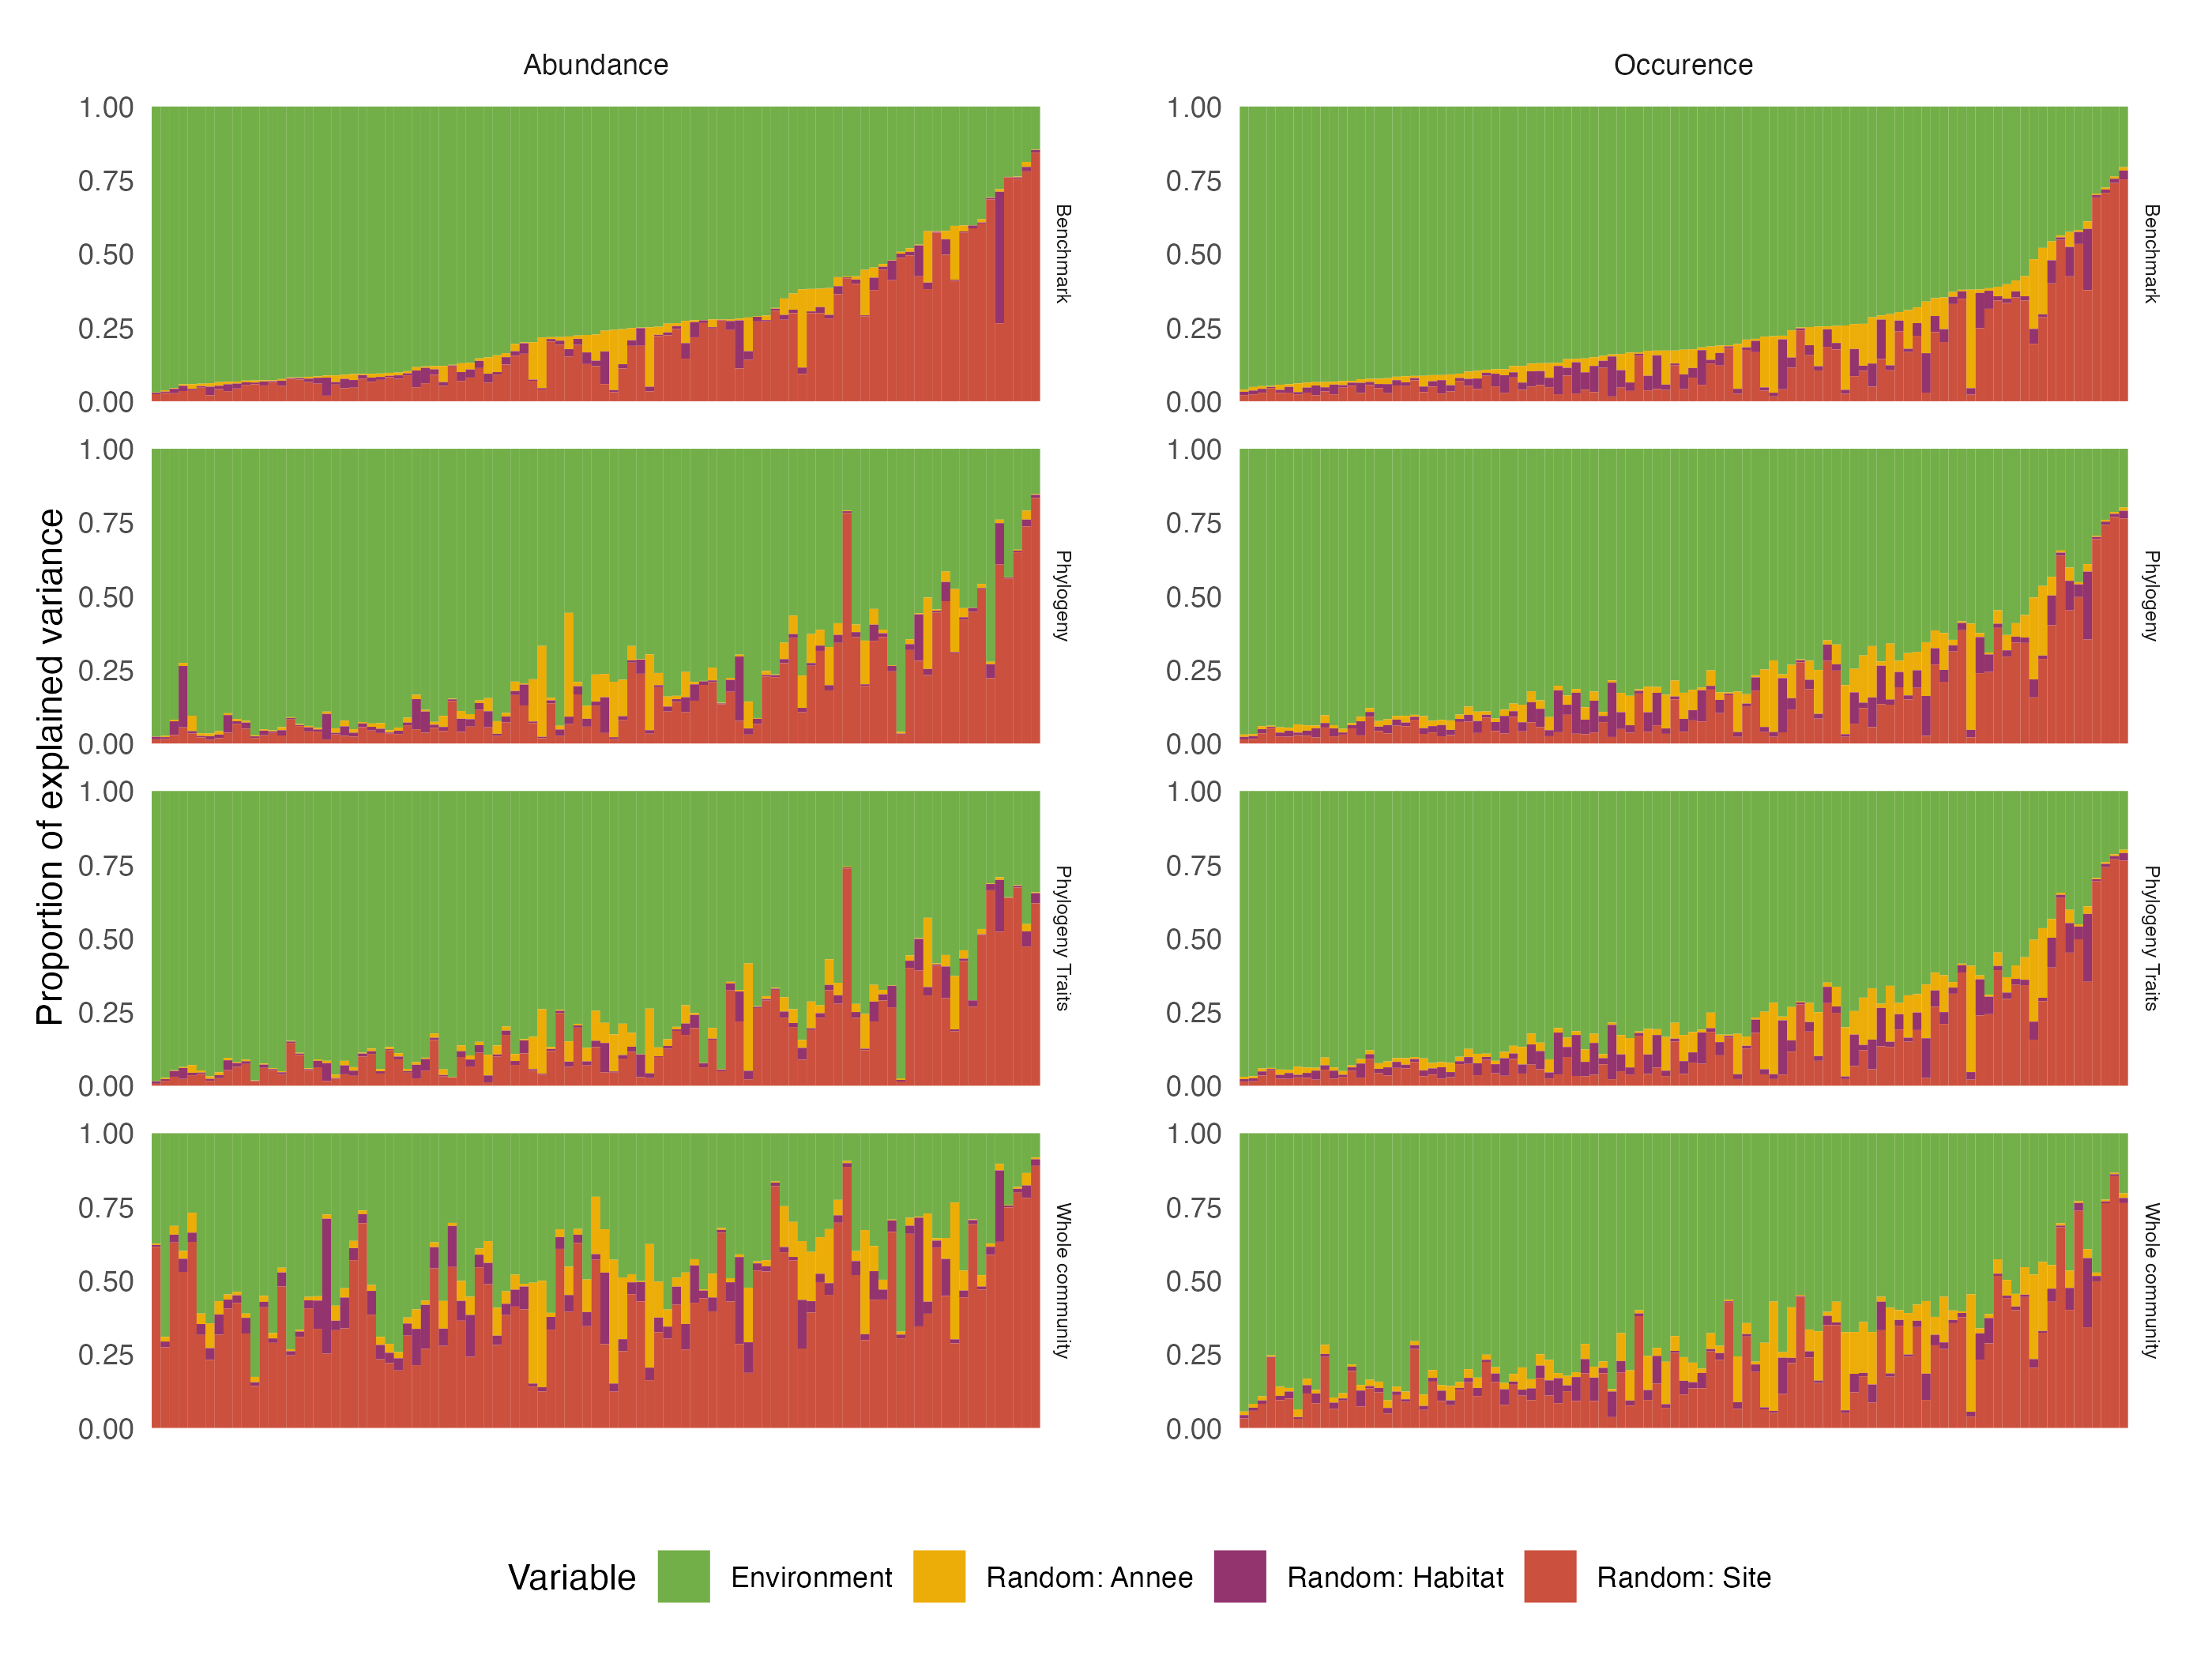
\includegraphics{04-Conclusion/figures/habitat_hmsc_random_effect.png}
\caption{Comparaison entre les quatre structures de modèle alternatives
étudiées dans le premier chapitre de cette thèse. Le graphique présente
pour chaque espèce (le long de l'axe des x) la variance qui est
expliquée (le long de l'axe y) par (1) les variables environnementales
(Environnement) et (2) les trois effets aléatoires. Les résultats sont
présentés pour les modèles ajustés aux données d'abondance (à gauche) et
de présence/absence (à droite). Les espèces sont classées par ordre
décroissant de variance expliquée par l'environnement pour le modèle de
référence.}\label{fig:disccusion1}
}
\end{figure}

\clearpage

\hypertarget{analyse-des-uxe9tats-dhabitats-marins-uxe0-luxe9chelle-du-globe-avancuxe9es-et-perspectives}{%
\section{Analyse des états d'habitats marins à l'échelle du globe :
avancées et
perspectives}\label{analyse-des-uxe9tats-dhabitats-marins-uxe0-luxe9chelle-du-globe-avancuxe9es-et-perspectives}}

L'identification des états d'habitats à l'échelle du globe constitue une
avancée en écologie en nous permettant de mieux caractériser les
habitats à ces grandes échelles et nous donnant une indication sur leur
état de santé. Cependant, l'approche mise en place dans cette thèse
n'éclaire pas sur l'état de santé des communautés que ces états
d'habitats abritent. En exploitant une approche de groupement,
\emph{HDBSCAN} \autocite{McInnes2017}, associée à une nouvelle technique
de réduction de dimension \emph{UMAP} \autocite{McInnes_2020}, j'ai
discerné plusieurs ensembles distincts, que j'ai définis comme des
``états d'habitat''. Ces états d'habitats se distinguent par leur
composition variée en espèces végétales (fucoïdes, laminaires, algues
brunes, rouges, etc.) et animales (invertébrés sessiles, coraux
branchus, coraux mous, gorgones\ldots), ainsi que par la présence de
divers substrats nus (comme le sable, le gravier ou la roche nue). Ces
états d'habitats apportent un éclairage nuancé sur l'état de santé des
zones dans lesquelles on les trouve, car, parmi ces ensembles, certains
correspondent à des habitats emblématiques (tels que les coraux branchus
ou les forêts de laminaires), tandis que d'autres représentent des états
dégradés ou des états alternatifs (Fig.~\ref{fig:chap2fig6}). Nos
recherches, élaborées dans les chapitres 2 et 3, révèlent que les
régions de transition entre les zones tempérées et tropicales, en
particulier le long des côtes est et ouest de l'Australie, exhibent une
plus forte richesse d'états d'habitats. Ces zones, actuellement en cours
de tropicalisation (processus où les espèces typiques des eaux tempérées
cèdent la place à des espèces tropicales ; \textcite{Verges_2014} ;
\textcite{Verges_2019}), pourraient être à l'aube d'un changement de
régime. Ces changements de régime sont probablement en train de se
produire actuellement, puisque nos observations indiquent une
homogénéisation progressive des fonds marins, caractérisée par la
prédominance croissante de l'état d'habitat ``turf'' depuis le milieu
des années 2010, un phénomène qui corrobore les études antérieures
menées sur les côtes australiennes \autocite{Pessarrodona_2022}, et les
tendances en cours à échelle globale \autocite{Filbee-Dexter_2018}.

\clearpage

\hypertarget{implications-des-travaux-entrepris-dans-cette-thuxe8se}{%
\section{Implications des travaux entrepris dans cette
thèse}\label{implications-des-travaux-entrepris-dans-cette-thuxe8se}}

Les travaux réalisés au cours de cette thèse ont non seulement marqué
certaines avancées méthodologiques, mais ont également enrichi notre
compréhension des habitats benthiques à l'ère de l'Anthropocène. Dans le
premier chapitre, j'ai élaboré un cadre d'analyse adaptée aux modèles
\emph{SDM} et \emph{jSDM}, facilitant et standardisant l'analyse de ces
modèles et de leur capacité à inférer les déterminants et à prédire les
multiples facettes de la biodiversité. Appliqué à un jeu de données de
suivi long-terme de la macrofaune au sein de deux habitats marins
côtiers à une échelle régionale, cette analyse a clarifié les mécanismes
d'assemblages de ces communautés. Les différents modèles réalisés ont
confirmé une influence limitée des filtres environnementaux sur ces
communautés (peu d'influence des variables évaluées, peu de lien avec
les traits des espèces) et mis en lumière pour la première fois dans ces
habitats un rôle important des co-occurrences entre espèces, qu'il
conviendra d'examiner plus en détail. Cette analyse a aussi mis en avant
les limites de ce cadre de modélisation pour des communautés riches,
dont les principaux déterminants ne semblent pas être les filtres
abiotiques, mais des processus neutres \autocite{Boye_2019a} ou des
processus biotiques (interactions entre espèces). Poursuivant cet élan,
les chapitres suivants ont introduit des méthodes novatrices de
réduction de dimension des données et de groupement pour analyser les
données en écologie et décrypter la complexité des habitats, notamment
en étudiant leurs patrons de distribution à l'échelle du globe. Cette
exploration a levé le voile sur les facteurs environnementaux et
anthropiques qui influencent la distribution des habitats et de leurs
états, fournissant ainsi des clés pour interpréter et projeter les
transformations futures de ces habitats biogéniques dans un contexte
d'environnement changeant dû à l'anthropocène. Les résultats de ces
recherches indiquent notamment une homogénéisation des habitats avec un
accroissement de la couverture du ``turf''.

En somme, cette thèse souligne le rôle crucial des habitats biogéniques
pour les écosystèmes marins et fournit de nouveaux outils pour mieux
comprendre et prédire à la fois leur réponse aux changements
environnementaux et les impacts en cascade que cela peut générer sur la
faune qui leur est associée. Considérant les services essentiels que ces
systèmes fournissent à l'humanité, ainsi que la valeur écologique
intrinsèque des habitats biogéniques, les résultats de ces recherches
mettent en relief la dégradation et la disparition de ces habitats
biogéniques comme une très forte menace pesant sur les écosystèmes
\autocite{ipbes_2019}. En réponse, l'urgence de programmes de
surveillance étendus, tant dans l'espace que dans le temps, est
indéniable pour mieux comprendre le fonctionnement des écosystèmes
marins et l'importance des habitats sur la structure des communautés,
notamment pour mieux appréhender les perturbations écologiques futures
liées à l'impact anthropique.

\clearpage

\printbibliography[heading=subbibintoc, title={Bibliographie}]
\end{refsection}